\documentclass[
	%parspace, % Térköz bekezdések közé / Add vertical space between paragraphs
	%noindent, % Bekezdésének első sora ne legyen behúzva / No indentation of first lines in each paragraph
	%nohyp, % Szavak sorvégi elválasztásának tiltása / No hyphenation of words
	%twoside, % Kétoldalas nyomtatás / Double sided format
	%final, % Teendők elrejtése / Set final to hide todos	
]{elteikthesis}[2020/02/26]
\usepackage{fancyhdr}
\usepackage{enumitem}
\renewcommand{\headrulewidth}{0.5pt}
\fancyheadoffset{\marginparwidth - 3.00cm}

% Dolgozat metaadatai
% Document's metadata
\title{Bevezetés a programozás világába} % cím / title
\date{2020} % védés éve / year of defense

% Szerző metaadatai
% Author's metadata
\author{Csonka Szilvia}
\degree{programtervező informatikus BSc}

% Témavezető(k) metaadatai
% Superivsor(s)' metadata
\supervisor{} % belső témavezető neve / internal supervisor's name
\affiliation{} % belső témavezető beosztása / internal supervisor's affiliation
%\extsupervisor{Külső Kornél} % külső témavezető neve / external supervisor's name
%\extaffiliation{informatikai igazgató} % külső témavezető beosztása / external supervisor's affiliation

% Egyetem metaadatai
% University's metadata
\university{Eötvös Loránd Tudományegyetem} % egyetem neve / university's name
\faculty{Informatikai Kar} % kar neve / faculty's name
\department{Algoritmusok és Alkalmazásaik Tanszék} % tanszék neve / department's name
\city{Budapest} % város / city
\logo{title} % logo

\usepackage{hyperref}
\usepackage{stuki}


% A dolgozat
% The document
\begin{document}

% Nyelv kiválasztása
% Set document language
\documentlang{magyar}
%\documentlang{english}

% Teendők listája (final dokumentumban nincs)
% List of todos (not in the final document)
%\listoftodos[\todolabel]

% Dokumentum beállítások
% Some document settings
% Lábjegyzet folytonos számozása fejezetek között
% Continuous counting of footnotes among chapters
\counterwithout{footnote}{chapter}

% Tartalomjegyzék oldalszámozásának rejtése
% Hide page numbering of ToC
\newcounter{conpageno}
\let\oldtableofcontents\tableofcontents
\renewcommand{\tableofcontents}{
	\pagenumbering{gobble}
	\oldtableofcontents
	\cleardoublepage
	\setcounter{conpageno}{\value{page}}
	\pagenumbering{arabic}
	\setcounter{page}{\value{conpageno}}
}


% Címlap (kötelező)
% Title page (mandatory)
\maketitle

% Tartalomjegyzék (kötelező)
% Table of contents (mandatory)
\tableofcontents
\cleardoublepage

% Tartalom
% Main content
\chapter{Előszó} % Introduction
\label{ch:intro}

Ezen anyagok, leírások célja, hogy betekintést mutasson a programozás világába olyanok számára, akik bár nem rendelkeznek programozási előismeretekkel, de érdekli őket a téma, és nem tudják, hogyan is láthatnának neki önállóan.

Az alábbi ismertető feladatok megoldásához ingyenesen letölthető, különösebb gép igénnyel nem rendelekező eszközökre lesz majd szükséged.

Az alábiakban a c++ programozási nyelvet és a code::blocks fejlesztői környezetet fogjuk használni.

A c++-t azért tartom alkalmasnak erre a célra, mert bár egy roppant bonyolult és sokszor nehezen érthető nyelvről van szó, azonban ez egy ún. multiparadigmás programozási nyelv (ennek jelentését később tárgyaljuk), mely lehetővé teszi, hogy egészen egyszerű kis programokat is írhassunk segítségével, nincs szükség hozzá semmilyen mélyebb tudásra, nincs semmi olyan, ami megbonyolítaná egy teljesen kezdő számára a használatot. Ugyan akkor egy nagyon populáris programozási nyelvről van szó, így akár a későbbiekben is hasznos tudás lehet ennek ismerete. 

A code::blocks fejlesztői környezetet azért tartom alkalmasnak kezdők számára, mivel a telepítését követően viszonylag könnyen használható, segítségével fordíthatjuk és futtathatjuk is a programunkat néhány kattintással, így kezdetben nem szükséges konzolból végezni ezeket, koncentrálhatunk a programozás alapjainak elsajátítására.

Célunk, hogy akár egy emelt szintű informatikai érettségire is fel lehessen készülni ezen anyagok alapján, vagy legalábbis egyfajta ugródeszkaként szolgáljon a programozáshoz, annak elkezdéséhez.
\cleardoublepage

\chapter{Bevezetés} % User guide
\label{ch:bevezetes}

\section{A szükséges programok telepítése}

\subsection{A telepítő letöltése}
Code::blocks fejlesztői környezetre és c++ compiler-re (fordító program) lesz szükségünk, amelyeket egy csomagban le is tölthetünk és telepíthetünk a code::blocks oldaláról: \url{https://sourceforge.net/projects/codeblocks/}. Jelenleg erről a linkről windows-ra tölthetjük le a code::blocks-ot c++ fordító programmal együtt. 

Ez a legfrisebb code::blocks verzió, amely jelenleg szerepel az érettségi során használható programok listáján. (Ha érettségire készülünk, ellenőrizzük, hogy olyan verziót telepítsünk, amelyet majd használhatunk is az érettségi során, így véletlenül sem érhet meglepetés bennünket azon okból, hogy a mi verziónk eltérő attól, mint amit majd ott használhatunk.)

Amennyiben valami miatt ez a link nem működne, \url{https://www.codeblocks.org/downloads/} linken válasszuk ki a "Download the binary release" menüpontot.

\begin{figure}[H]
	\centering
	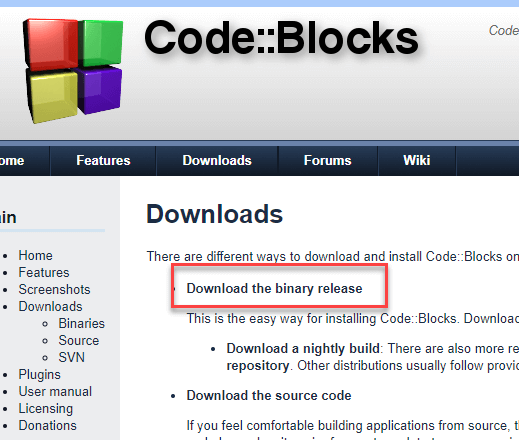
\includegraphics[width=0.5\linewidth]{images/bevezetes/choose}
	\caption{"Download the binary release"}
	\label{fig:choose}
\end{figure}

Ezt követően válasszuk ki a gcc compiler-rel való letöltését az intaller-nek.

\begin{figure}[H]
	\centering
	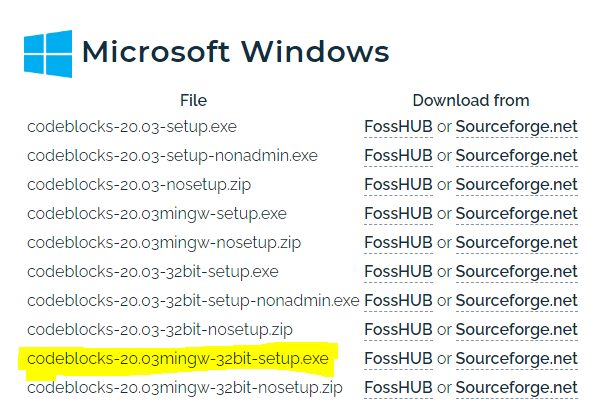
\includegraphics[width=0.8\linewidth]{images/bevezetes/download_installer}
	\caption{"Code::blocks telepítő gcc fordítóprogrammal való letöltése"}
	\label{fig:choose}
\end{figure}

\subsection{Telepítés}

A telepítő letöltését követően futtassuk azt. Mindent hagyjuk az alap beállításon, és navigáljunk keresztül a telepítőn. Esetleg a telepítés helyét módosíthatjuk, ha szeretnénk.

\subsection{A program üzembe helyezése}

A telepítést követően felajánlja számunkra a program elindítását a telepítő, javaslom, ezzel éljünk is. Az első indításnál ha minden jól megy, érzékeli is a program a fordító programot, amelyet a code::blocks-al együtt telepítettünk.

\begin{figure}[H]
	\centering
	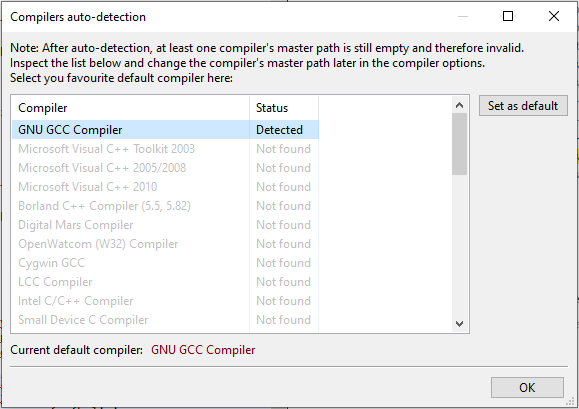
\includegraphics[width=1.0\linewidth]{images/bevezetes/set_compiler}
	\caption{Alapértelmezett fordítóprogram beállítása}
	\label{fig:choose}
\end{figure}

Válasszuk is ki a GNU GCC Compiler-t (ezt a fordítóprogramot telepítettük az imént a code::blocks-al együtt), menjünk a "Set as default"-ra (beállítás alapértelmezettként), majd kattintsuk az "OK"-ra.

Ezt követően megnyílik a program, és valószínűleg ismét egy felugró ablakba botlunk, amely arról érdeklődik, hogy szeretnénk-e bizonyos fájltípusok megnyitásához alapértelmezettként a code::blocks-ot rendelni. Ez azért lehet hasznos, mivel a későbbiekben egyszerűben dupla kattintással megnyithatjuk majd a projektjeinket, nem kell majd először a code::blocks-ot megnyitni, majd külön a programon belül kiböngészni a projektünket és úgy nyitni meg.

Én javaslom az alábbi menüpont kiválasztását.

\begin{figure}[H]
	\centering
	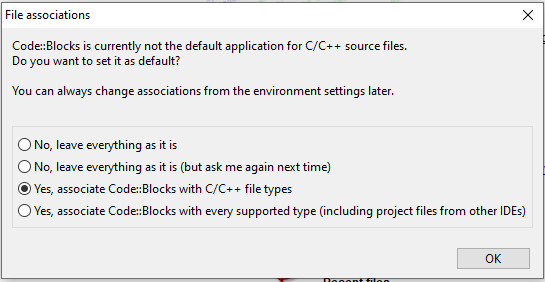
\includegraphics[width=0.7\linewidth]{images/bevezetes/associate_code_blocks}
	\caption{A c/c++ fájlok automatikusan code::blocks-al nyíljanak meg}
	\label{fig:choose}
\end{figure}

Ha minden igaz, ezt követően már használhatjuk is kisebb c++ projektek elkészítéséhez fejlesztői környezetünket, azonban ajánlom leellenőrizni a fordítóprogram beállításait: gyakori hiba kezdetben a code::blocks-nál, hogy nem találja azt, emiatt nem tudja lefordítani a forráskódjainkat.

Válasszuk ki a fejlécben a "Settings"-t majd a legördülő menüben a "Compiler"-t.


\begin{figure}[H]
	\centering
	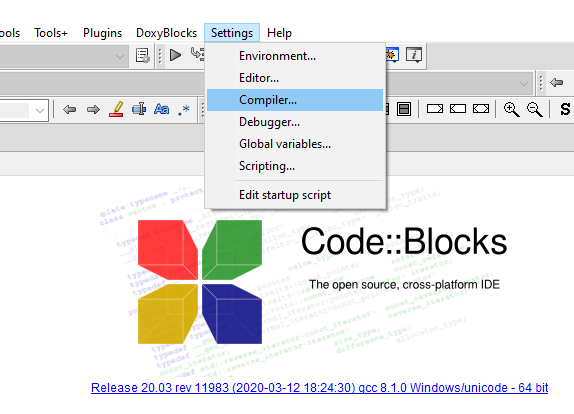
\includegraphics[width=0.7\linewidth]{images/bevezetes/check_compiler_01}
	\caption{A fordítóprogram beállításainak ellenőrzése}
	\label{fig:choose}
\end{figure}

Ezt követően a felugró ablak felső részében elhelyezkedő menüpontok közül válasszuk ki a "Toolchain executables"-t. Itt a fordítóprogram helyének kell lennie. Amennyiben minden jól ment, itt már szerepel egy elérési útvonal, ha a telepítés helyét a default-on hagytuk, akkor pontosan oda hivatkozik, ahova az a képen is látható.

\begin{figure}[H]
	\centering
	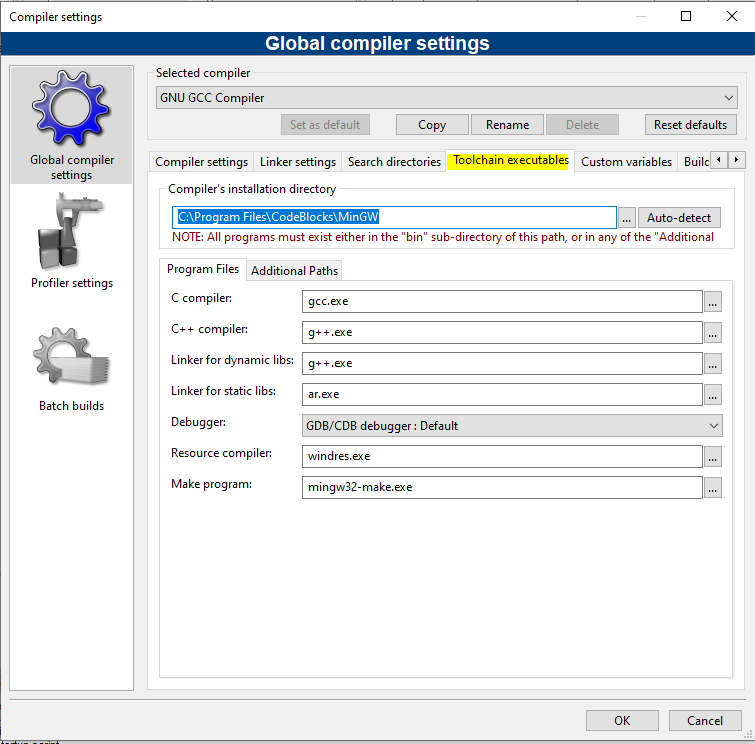
\includegraphics[width=1.0\linewidth]{images/bevezetes/check_compiler_02}
	\caption{A fordítóprogram helyének ellenőrzése}
	\label{fig:choose}
\end{figure}

Ha szeretnénk beállítani, hogy a c++ mely standard-ját szeretnénk használni (bizonyos években "frissítik" a programozási nyelveket is, akár a programokat, de jó esetben az újítások után is használhatóak lesznek a régebbi megoldások is), azt szintén itt, a "Compiler settings" almenüben tehetjük meg.

\begin{figure}[H]
	\centering
	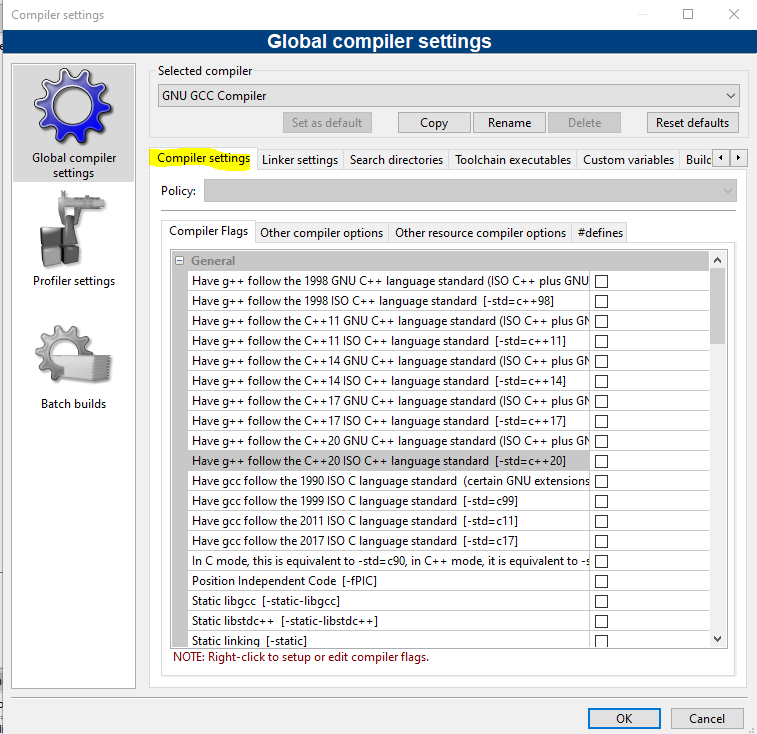
\includegraphics[width=1.0\linewidth]{images/bevezetes/check_compiler_03}
	\caption{A fordítóprogram standard-jának ellenőrzése}
	\label{fig:choose}
\end{figure}

Ahogyan azt a képen is láthatjuk, a 2020-as standard a legfrissebb jelenleg. Jómagam azt javaslom, hogy amennyiben érettségire készülünk, válasszuk a legfrissebb olyan standard-et, amelyet ott is használhatunk, amennyiben nem, válasszuk a legfrissebbet.

\section{Alapvető fogalmak}

Ebben a részben olyan fogalmak jelentését fogjuk tisztázni, amelyek a legtöbbször előfordulnak, ha programozásról van szó, esetleg a korábbiakban is említésre kerültek már.

\paragraph{Programozási nyelv}
A programozási nyelv célja, hogy olyan módon írhassuk le programok működését, amely emberek számára is olvasható, megérthető, jól strukturált, és egyértelmű. Azonban ezek a számítógép számára alapból nem értelmezhetőek, ezért szükséges fordító program (compiler) használata, amely gépi kódra, azaz a számítógép számára értelmezhető, futtatható formába alakítja azt át. A programozási nyelvek között vannak ún. alacsonyabb és magasabb szintűek. Az alacsonyabb szintűek közelebb állnak a gépi kódhoz, a magasabb szintűek pedig távolabb, ezek segítségével álltalában bonyolultbb logikájú, stukturáltabb programokat írhatunk. Ilyen magasabb szintű programozási nyelv többek között a c++ is. Programozóként nem nagyon fogunk alacsony szintű programozási nyelvekkel találkozni. Bővebben lásd: \url{https://hu.wikipedia.org/wiki/Programoz%C3%A1si_nyelv}.

\paragraph{Fordítóprogram} A fordítóprogram olyan program, amely valamely programozási nyelvben írt programot gépi kódra, számítógép által értelmezhető, futtatható formára alakít át. Bővebben lásd.: \url{https://hu.wikipedia.org/wiki/Ford%C3%ADt%C3%B3program}.

\paragraph{Fejlesztői környezet}
Olyan program (ez lehet bármi egyéb is, de az egyszerűség kedvéért gondoljunk most programra), amely funkcióival segíti a programozó dolgát: például megjeleníti a programkódot, ily módon ez lehet egy egyszerű jegyzettömb is. Kicsit bonyolultabb fejlesztői környezet például a code::blocks is, bár ez azért jóval több funkciót kínál, mint egy egyszerű jegyzettömb. Például segítségével lefordíthatjuk és futtathatjuk is programunkat. A programkódot sem egyszerűen, hanem ún. "syntax highlight"-al jeleníti meg. Ez egyszerűen annyit takar, hogy bizonyos kulcsszavakat különböző színűre színez, így átláthatóbb a kód. Bővebben lásd.: \url{https://hu.wikipedia.org/wiki/Fejleszt%C5%91i_k%C3%B6rnyezet}.

\paragraph{Forrásfájl}
Olyan fájl, amely a program kódját tartalmazza. Nagyobb programok álltalában több forrásfájlból állnak.

\paragraph{Forráskód} A program még le nem fordított állapotban lévő kódja, amelyet a forrásfájlok tartalmaznak (nagyobb programok esetén ez több forrásfájlból áll). Ez nem futtható, csak fordítás után. (Amelyet a fordítóprogram, angol kifejezéssel compiler [kompájler] végez el.) Ha egy program forráskódja a rendelkezésünkre áll, akkor azt továbbfejleszthetjük, esetleg funkcióit módosíthatjuk segítségével. Ezt a bináris (gépi kód) verzión nem tehetjük meg. Ezért tulajdonképpen ez a program lelke.

\section{Az első programom}

\cleardoublepage

\chapter{Példa} % Developer guide
\label{ch:impl}


\begin{lstlisting}
int 5 = 2;
\end{lstlisting}
\begin{center}
	\begin{longtable}{ | m{0.20\textwidth} | 	m{0.30\textwidth} |m{0.40\textwidth}| }
		\hline
		\textbf{Én mint \newline \textit{(As a)}} & \textbf{Szeretnék \newline \textit{(Want)}} & \textbf{Azért hogy \newline \textit{(So that)}} \\
		\hline \hline
		
		Vendég & Játékok listázása. & Azért, hogy láthassam azokat a kalandjátékokat, amelyekhez megtekintési joggal rendelkezem. \\
		\hline
		
		Vendég & Regisztráció a weboldalra. & Azért, hogy igénybe vehessem az alkalmazás azon szolgáltatásait is, amelyekhez autentikáció szükséges. \\
		\hline
		
		Vendég &  Bejelentkezés a weboldalra. & Azért, hogy elérhessem korábban felvett, egyéni adataimat, fiókomat.\\
		\hline
		
		Bejelentkezett felhasználó & Kijelentkezés a weboldalról. & Azért, hogy a böngészőm ne tárolja bejelentkezésem adatait.\\
		\hline
		
		Bejelentkezett felhasználó & Regisztráció törlése.& Azért, hogy korábban felvett egyéni adataim ne legyenek többé elérhetőek, a weboldal adatbázisából törlődjenek.\\
		\hline
		
		Bejelentkezett felhasználó & Fiók adatok módosítása. & Azért, hogy módosíthassam a regisztráció során megadott adataimat.\\
		\hline
		
		Bejelentkezett felhasználó & Új kalandjáték létrehozása. & Azért, hogy új kalandjátékkal bővítsem saját játékaimat.\\
		\hline
		
		Bejelentkezett felhasználó & Már meglévő kalandjáték módosítása. & Azért, hogy módosíthassam a korábban létrehozott kalandjátékom adatait.\\
		\hline
		
		Bejelentkezett felhasználó & Saját kalandjáték törlése. & Azért, hogy törölhessem korábban létrehozott kalandjátékom adatait. \\
		\hline
		
		Bejelentkezett felhasználó & Játékmenet indítása. & Azért, hogy játszhassak a számomra elérhető kalandjátékok valamelyikével.\\
		\hline
		
	\caption{Felhasználói történetek.}
	\label{user_storys}
	\end{longtable}
\end{center}


\cleardoublepage

\chapter{Tesztelés} % User guide
\label{ch:test}

\cleardoublepage

\chapter{Összegzés} % Conclusion
\label{ch:sum}


\cleardoublepage



\chapter{Hivatkozások} 




\cleardoublepage


% Függelékek (opcionális) - hosszabb részletező táblázatok, sok és/vagy nagy kép esetén hasznos
% Appendices (optional) - useful for detailed information in long tables, many and/or large figures, etc.
%\appendix
%\chapter{Szimulációs eredmények} % Simulation results
\label{appx:simulation}

Lorem ipsum dolor sit amet, consectetur adipiscing elit. Pellentesque facilisis in nibh auctor molestie. Donec porta tortor mauris. Cras in lacus in purus ultricies blandit. Proin dolor erat, pulvinar posuere orci ac, eleifend ultrices libero. Donec elementum et elit a ullamcorper. Nunc tincidunt, lorem et consectetur tincidunt, ante sapien scelerisque neque, eu bibendum felis augue non est. Maecenas nibh arcu, ultrices et libero id, egestas tempus mauris. Etiam iaculis dui nec augue venenatis, fermentum posuere justo congue. Nullam sit amet porttitor sem, at porttitor augue. Proin bibendum justo at ornare efficitur. Donec tempor turpis ligula, vitae viverra felis finibus eu. Curabitur sed libero ac urna condimentum gravida. Donec tincidunt neque sit amet neque luctus auctor vel eget tortor. Integer dignissim, urna ut lobortis volutpat, justo nunc convallis diam, sit amet vulputate erat eros eu velit. Mauris porttitor dictum ante, commodo facilisis ex suscipit sed.

Sed egestas dapibus nisl, vitae fringilla justo. Donec eget condimentum lectus, molestie mattis nunc. Nulla ac faucibus dui. Nullam a congue erat. Ut accumsan sed sapien quis porttitor. Ut pellentesque, est ac posuere pulvinar, tortor mauris fermentum nulla, sit amet fringilla sapien sapien quis velit. Integer accumsan placerat lorem, eu aliquam urna consectetur eget. In ligula orci, dignissim sed consequat ac, porta at metus. Phasellus ipsum tellus, molestie ut lacus tempus, rutrum convallis elit. Suspendisse arcu orci, luctus vitae ultricies quis, bibendum sed elit. Vivamus at sem maximus leo placerat gravida semper vel mi. Etiam hendrerit sed massa ut lacinia. Morbi varius libero odio, sit amet auctor nunc interdum sit amet.

Aenean non mauris accumsan, rutrum nisi non, porttitor enim. Maecenas vel tortor ex. Proin vulputate tellus luctus egestas fermentum. In nec lobortis risus, sit amet tincidunt purus. Nam id turpis venenatis, vehicula nisl sed, ultricies nibh. Suspendisse in libero nec nisi tempor vestibulum. Integer eu dui congue enim venenatis lobortis. Donec sed elementum nunc. Nulla facilisi. Maecenas cursus id lorem et finibus. Sed fermentum molestie erat, nec tempor lorem facilisis cursus. In vel nulla id orci fringilla facilisis. Cras non bibendum odio, ac vestibulum ex. Donec turpis urna, tincidunt ut mi eu, finibus facilisis lorem. Praesent posuere nisl nec dui accumsan, sed interdum odio malesuada.
%\cleardoublepage

% Irodalomjegyzék (kötelező)
% Bibliography (mandatory)
% Ábrajegyzék (opcionális) - 3-5 ábra fölött érdemes
\addcontentsline{toc}{chapter}{\lstfigurelabel}
\listoffigures
\cleardoublepage

% Táblázatjegyzék (opcionális) - 3-5 táblázat fölött érdemes
% List of tables (optional) - useful over 3-5 tables
\addcontentsline{toc}{chapter}{\lsttablelabel}
\listoftables
\cleardoublepage


% Jelölésjegyzék (opcionális)
% List of symbols (optional)
%\printnomenclature

\end{document}
